\section{Caractéristiques d'un dipôle (3 points)}

Pierre a tracé le graphique caractéristique d'une résistance.

\begin{center}
	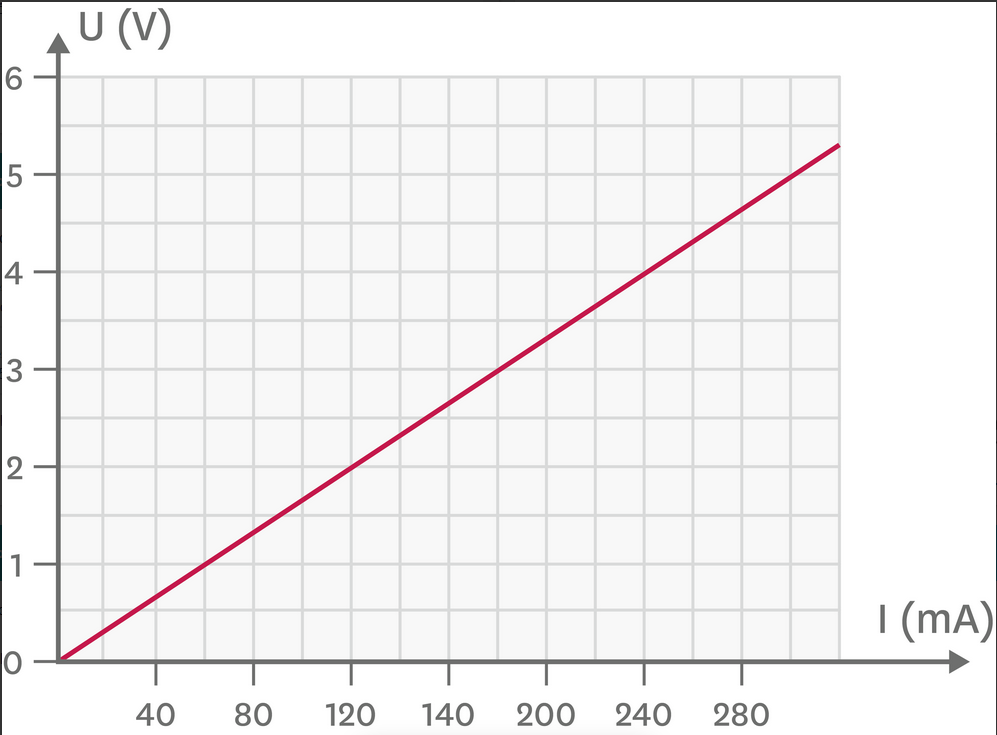
\includegraphics[scale=0.35]{img/graph}
\end{center}

\begin{questions}
	\question[1] Quelle est la tension aux bornes de la résistance lorsqu'elle est traversée par un courant d'intensité 60 $mA$ ?
	\begin{solution}
		Lorsqu'elle est traversée par un courant d'intensité 60 $mA$, la tension aux bornes de la résistance est 1 $V$.
	\end{solution}
	
	\question[1] Quelle est l'intensité du courant  dans la résistance si la tension à ses bornes est égale à 5 $V$ ?
	\begin{solution}
		Si la tension aux bornes de la résistance est égale à 5 $V$, elle est traversée par un courant de 300 $mA$.
	\end{solution}
	
	\question[1] Quelle est la valeur de cette résistance ?
	\begin{solution}
		D'après la loi d'Ohm, aux bornes de la résistance on a :
		
		\begin{eqnarray*}
			U &=& R \times I \\
			R &=& \frac{U}{I}\\
			R &=& \frac{1}{\num{0.3}}\\
			R &\approx& \num{3.33} \\
		\end{eqnarray*}
	
	Donc la valeur de cette résistance est \num{3.33} $\Omega$.
	\end{solution}
\end{questions}